\section{Run log and setup}
\label{app:runlog}

Table~\ref{tab:cells} lists the \NCells{} cells and the CPU control of Appendix~\ref{app:cpucontrol} with the date each one started and its host CPU, and Table~\ref{tab:setup} lists the software and hardware, read from the metadata that every cell records. In order: the reference cells ran on \RefDates; our record dates the decision rule to \RuleDate; the pilot ran on \PilotDate; the rerun and variant cells on \VariantDates; the open-loop check on \OlDates; and the CPU control on \CpuCtrlDates.

% Generated by scripts/make_assets.py from run_meta.json and the episode records of every cell.
\begin{table}[t]
\caption{The twelve cells of the study and their run log. Each cell runs the 500 (task, initial state) pairs of LIBERO-Spatial. Date: day of 2026 on which the cell started; hours: summed episode time on one GPU (not logged by the original OpenVLA-OFT script); host CPU as recorded in the run metadata (the two reference cells ran with the original scripts, which do not record it). Every cell ran on one NVIDIA RTX PRO 4500 Blackwell GPU.}
\label{tab:cells}
\centering
\scriptsize
\setlength{\tabcolsep}{3pt}
\begin{tabular}{@{}llL{0.36\columnwidth}lrl@{}}
\toprule
Model & Cell & What changes & Date & Hours & Host CPU \\
\midrule
OpenVLA-7B & Reference & original evaluation script, unchanged & 6 Oct & 5.2 & not logged \\
 & Rerun (A/A) & reference repeated unchanged & 28 Oct & 4.6 & EPYC 7663 \\
 & JPEG off & no JPEG round trip before the resize & 28 Oct & 4.5 & EPYC 7663 \\
 & Crop step off & no center crop (script flag) & 28 Oct & 4.6 & EPYC 7663 \\
 & Bilinear resize & bilinear instead of Lanczos3 resize & 29 Oct & 4.7 & EPYC 7663 \\
 & Render at 224 & cameras rendered at 224, not 256 & 29 Oct & 4.2 & EPYC 7443 \\
\midrule
OpenVLA-OFT & Reference & original evaluation script, unchanged & 3 Oct, 5 Oct & - & not logged \\
 & Rerun (A/A) & reference repeated unchanged & 29 Oct & 0.7 & EPYC 7663 \\
 & JPEG off & no JPEG round trip before the resize & 29 Oct & 0.7 & EPYC 7663 \\
 & Crop step off & no center crop (script flag) & 29 Oct & 0.7 & EPYC 7763 \\
 & Bilinear resize & bilinear instead of Lanczos3 resize & 29 Oct & 0.6 & EPYC 7663 \\
 & Render at 224 & cameras rendered at 224, not 256 & 29 Oct & 0.7 & EPYC 7663 \\
\bottomrule
\end{tabular}
\end{table}

% Generated by scripts/make_assets.py from run_meta.json of the cells.
\begin{table}[t]
\caption{Evaluation setup, read from the run metadata that every cell records.}
\label{tab:setup}
\centering
\footnotesize
\begin{tabular}{@{}L{0.22\columnwidth}L{0.71\columnwidth}@{}}
\toprule
Item & Value \\
\midrule
Checkpoints & \path{openvla/openvla-7b-finetuned-libero-spatial}; \path{moojink/openvla-7b-oft-finetuned-libero-spatial} \\
Episodes & LIBERO-Spatial, 10 tasks $\times$ 50 stored initial states = 500 per cell; 10 settle steps + at most 220 policy steps \\
Simulator & MuJoCo 3.3.7, robosuite 1.4.1, headless offscreen rendering (EGL) \\
Libraries & PyTorch 2.8.0, Transformers 4.40.1, TensorFlow 2.16.2, NumPy 1.26.4 \\
Model settings & seed 7, environment seed 0, scaled dot-product attention (SDPA), greedy decoding (OpenVLA-7B); chunks of 8 actions (OpenVLA-OFT) \\
Code & OpenVLA commit \texttt{c8f03f4}, OpenVLA-OFT commit \texttt{e4287e9}, LIBERO commit \texttt{8f1084e} \\
Hardware & one NVIDIA RTX PRO 4500 Blackwell (32 GB) per cell; host CPU per cell in Table~\ref{tab:cells} (EPYC 7663 for every harness cell except OpenVLA-OFT with the crop step off, EPYC 7763, and OpenVLA-7B rendered at 224, EPYC 7443) \\
Compute & 31 GPU hours for the 5,500 timed episodes of Table~\ref{tab:cells} (the original OpenVLA-OFT script does not log time) \\
\bottomrule
\end{tabular}
\end{table}


\subsection{Pilot cells}
\label{app:pilot}

Before the full variant cells, a pilot ran \PilotCells{} cells of \PilotPairs{} episodes on initial states \SplitA{} of every task, all on \PilotDate{} on one machine (Table~\ref{tab:pilot}): the reference, an identical rerun and JPEG off for both models, and the crop step off for OpenVLA-7B. Its JPEG-off comparison for OpenVLA-7B gave the share of flips, \PilotDisc\%, that the decision rule of Section~\ref{sec:stats} uses, and the pilot cells are compared with the full cells in the reproducibility check of Section~\ref{sec:repro}. The pilot is not pooled with the full cells, but its initial states are among theirs and the full cells repeat its outcomes, so \PilotPairs{} of the \NPairs{} pairs of the primary comparison were known before the full cells ran; Section~\ref{sec:effects} reports the other \OutPairs{} separately. The per-episode records and run metadata of the pilot cells are released with the paper source.

% Generated by scripts/make_assets.py from data/pilot_states_0-19/*/run_meta.json and episodes.jsonl.
\begin{table}[t]
\caption{The pilot cells, run before the full cells on initial states 0-19 of every task (200 episodes per cell). Start: day and time (clock of the cloud instance) at which the cell started, from its run metadata. Successes: of 200. Differ: outcomes that differ from the full cell of the same pipeline on the same 200 pairs. The pilot included two variant steps; it fixed the share of flips used by the decision rule and is not pooled with the full cells.}
\label{tab:pilot}
\centering
\footnotesize
\begin{tabular}{@{}llllrl@{}}
\toprule
Model & Cell & Start & Successes & Differ & Host CPU \\
\midrule
OpenVLA-7B & Reference & 12 Oct 02:20 & 161 & 0 & EPYC 7713P \\
 & Rerun (A/A) & 12 Oct 09:21 & 161 & 0 & EPYC 7713P \\
 & JPEG off & 12 Oct 04:26 & 168 & 0 & EPYC 7713P \\
 & Crop step off & 12 Oct 07:15 & 167 & 1 & EPYC 7713P \\
OpenVLA-OFT & Reference & 12 Oct 01:55 & 198 & 0 & EPYC 7713P \\
 & Rerun (A/A) & 12 Oct 06:52 & 198 & 0 & EPYC 7713P \\
 & JPEG off & 12 Oct 06:28 & 196 & 0 & EPYC 7713P \\
\bottomrule
\end{tabular}
\end{table}


\subsection{CPU control of the OpenVLA-OFT crop-off cell}
\label{app:cpucontrol}

The OpenVLA-OFT crop-off cell ran on an \CpuOftCrop{} host, while every other OpenVLA-OFT harness cell ran on an \CpuMain. We reran it on an \CpuCtrlCpu{} host, with the same split of initial states and the same configuration. The rerun succeeds on \CpuCtrlK{} of \NPairs{} episodes, and its outcome is the same as the original cell on \CpuCtrlSame{} of \NPairs{} initial states, which is the floor of the identical OpenVLA-OFT rerun on this stack. Against the reference cell it loses \CpuCtrlLost{} and gains \CpuCtrlGained{} episodes ($p = \CpuCtrlP$), as the original cell does. The host CPU therefore does not account for the result of the crop step on OpenVLA-OFT, and the original cell stays the reported result; the effect remains exploratory for the reasons given in Section~\ref{sec:effects}.\HookCpuAppendix{}

\subsection{Runs under MuJoCo \MujocoNewVersion}
\label{app:mujoco}

The motivating example of Section~\ref{sec:intro} comes from two reproduction runs made before this study: OpenVLA-7B on initial states \SplitA{} of every task under MuJoCo \MujocoNewVersion{} (\MujocoNewK{} of \PilotPairs, \MujocoNewPct\%, with \MujocoNewTaskFive{} of \PilotStates{} in task \TaskFive), and OpenVLA-OFT on task \TaskFive{} only (\OftNewTaskFive). Under MuJoCo \MujocoVersion{} the same \PilotPairs{} OpenVLA-7B episodes give \MujocoOldK{} (\MujocoOldPct\%), the outcomes of our reference cell on those states. Their per-task results and the OpenVLA-OFT log are released with the paper source; they record the checkpoint, the initial states and the GPU but not the full software stack, so the example shows how far an evaluation can move and is not a controlled comparison of simulator versions.

\section{Image-level measurements}
\label{app:eda}

\begin{figure}[t]
\centering
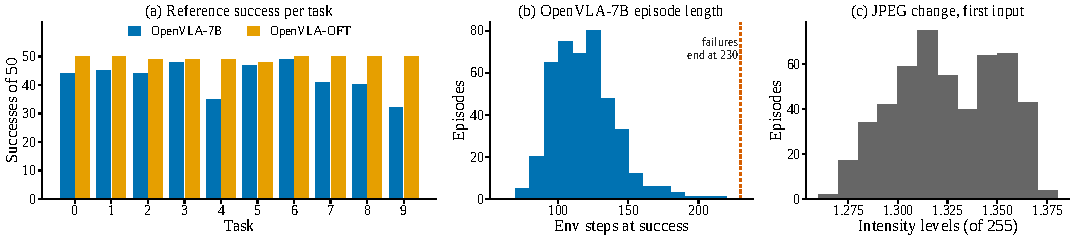
\includegraphics[width=\textwidth]{figures/data.pdf}
\caption{Data of the reference cells (\NPairs{} episodes per model). (a) Successes per task. (b) Number of environment steps at which successful OpenVLA-7B episodes end; failures always run to the limit of \MaxSteps{} (\SettleSteps{} settle steps plus \PolicySteps{} policy steps). (c) Mean absolute change that the JPEG round trip makes to the first resized image, before the crop, of each of the \NPairs{} OpenVLA-7B initial states, rendered on the GPU and logged by the JPEG-off cell, whose first frames equal those of every other harness cell.}
\label{fig:data}
\end{figure}

\paragraph{Outcomes.} Figure~\ref{fig:data}a shows the success of the reference cells per task. OpenVLA-7B ranges from \TaskMinSev{} to \TaskMaxSev{} of \NStates, with task \TaskNine{} (bowl on the wooden cabinet) and task \TaskFour{} (bowl in the top drawer) the hardest, while OpenVLA-OFT succeeds on \TaskMinOft{} to \TaskMaxOft{} in every task. Successful OpenVLA-7B episodes end after a median of \SuccStepMedian{} environment steps (interquartile range \SuccStepQone-\SuccStepQthree), well before the limit of \MaxSteps{} at which every failure ends (Figure~\ref{fig:data}b); whether a failed rollout would succeed later is unknown, but cutting the budget does not reduce the flips (Appendix~\ref{app:ablation}).

\paragraph{Size of the image changes.} On the GPU-rendered first frame of all \NPairs{} episodes, the JPEG round trip changes the resized image before the crop by \GpuMadMean{} intensity levels on average (range \GpuMadMin{} to \GpuMadMax, Figure~\ref{fig:data}c), and the bilinear kernel changes it by \GpuBilMean. The change is almost the same in every scene. To compare all steps on the final policy input, we rendered the first frame of the first \EdaStates{} initial states of every task on a CPU (\EdaFrames{} frames) and passed each through the official code with and without each change (Table~\ref{tab:eda}). On those frames the JPEG change before the crop is \CpuPreMean{} levels against \GpuSameMean{} for the same states on the GPU, so the CPU frames are representative. The bilinear kernel, the JPEG round trip and rendering at \InputRes{} change the policy input by \EdaBil, \EdaJpeg{} and \EdaRend{} levels on average; the JPEG change touches \EdaJpegChanged\% of the pixels. Turning the crop off is a different kind of change: it rescales and shifts the whole image, which gives a large per-pixel difference (\EdaCrop{} levels) although the content is the same. For scale, the mildest ImageNet-C JPEG corruption~\citep{imagenetc} changes the input by \EdaCone{} levels, and severity \ExtStableSevLo, which lowers OpenVLA from \ExtStableClean\% to \ExtStableJpegThree\% in StableVLA's evaluation~\citep{stablevla}, by \EdaCthree{} levels, \EdaCthreeRatio{} times the change of the JPEG step.

% Generated by scripts/make_assets.py from eda/frames.jsonl (scripts/eda_frames.py).
\begin{table}[t]
\caption{How far each change moves the $224 \times 224$ RGB policy input of OpenVLA-7B, against the input of the official pipeline. Mean: mean absolute difference over all pixels and the three color channels, in intensity levels (0-255), averaged over 50 first frames (initial states 0-4 of every task, rendered on CPU); range over frames; p99: 99th percentile of the per-value change; changed: share of pixels with any change. The four steps of this study are on top; the grayscale input and the ImageNet-C JPEG corruption are not part of any evaluation pipeline and are listed for scale.}
\label{tab:eda}
\centering
\footnotesize
\setlength{\tabcolsep}{3.5pt}
\begin{tabular}{@{}lrcrr@{}}
\toprule
Change & Mean & Range & p99 & Changed (\%) \\
\midrule
Bilinear resize & 0.64 & 0.59-0.70 & 8 & 40 \\
JPEG off & 1.26 & 1.21-1.30 & 6 & 96 \\
Render at 224 & 1.76 & 1.61-1.90 & 17 & 79 \\
Crop step off (rescales) & 8.33 & 7.74-8.96 & 102 & 88 \\
\midrule
Grayscale (luminance only) & 6.25 & 6.08-6.44 & 24 & 95 \\
ImageNet-C JPEG, sev.~1 (q.~25) & 3.44 & 3.31-3.59 & 18 & 99 \\
ImageNet-C JPEG, sev.~3 (q.~15) & 4.60 & 4.45-4.74 & 23 & 100 \\
ImageNet-C JPEG, sev.~5 (q.~7) & 7.65 & 7.49-7.86 & 32 & 100 \\
\bottomrule
\end{tabular}
\end{table}


\paragraph{Color inputs, and why no grayscale.} The policies always receive RGB images, in the reference and in every variant, and the intensity level is the average size of the change in the RGB values the policy receives, the same quantity as the mean absolute error used for image quality; it is not a grayscale conversion. We did not study grayscale inputs, for three reasons. Both checkpoints were trained on RGB frames, so a grayscale input would be a mismatch larger than any of the three steps that keep the geometry: replacing the policy input by its luminance changes it by \EdaGray{} intensity levels, about \EdaGrayRatio{} times the change of the JPEG round trip (Table~\ref{tab:eda}). Grayscale also removes the chroma that separates surfaces of similar brightness, and the policy has to find a particular black bowl among similar objects. And the question is which steps of the real evaluation pipeline must be matched, and grayscale is not one of them.

\section{Ablation of the analysis}
\label{app:ablation}

The variants themselves are an ablation of the evaluation pipeline: each removes or replaces one component and keeps the rest. Table~\ref{tab:ablation} ablates the choices of the analysis on the primary comparison and checks the reading of the secondary results.

% Generated by scripts/make_assets.py.
\begin{table}[t]
\caption{Ablation of the analysis choices on the primary comparison (JPEG off, OpenVLA-7B), and checks of the reading of the secondary results. Change and 95\% bootstrap interval in points; bound: one-sided 95\% upper bound on the loss.}
\label{tab:ablation}
\centering
\footnotesize
\setlength{\tabcolsep}{3pt}
\begin{tabular}{@{}L{0.45\columnwidth}L{0.49\columnwidth}@{}}
\toprule
Choice removed or changed & Result \\
\midrule
Paired bootstrap (as reported) & $-$0.8 [$-$4.2, +2.6], width 6.8, bound 3.6 \\
Pairing removed (cells treated as independent samples) & $-$0.8 [$-$5.2, +3.6], width 8.8, bound 4.6 \\
200 initial states (0-19) instead of 500 & +3.5 [$-$2.5, +9.5], width 12.0; 14 lost, 21 gained \\
One task left out (10 analyses) & change between $-$1.6 and $-$0.2 \\
Step budget cut from 230 to 180 / 150 / 120 env steps & flips 81 / 90 / 87 (against 74) \\
Initial states 20-49 only (outside the pilot) & $-$3.7 [$-$7.7, +0.3], bound 7.0; 25 lost, 14 gained, $p = 0.11$ \\
Tasks resampled instead of episodes & [$-$3.0, +1.6], bound 2.8 (OpenVLA-OFT crop off: [$-$5.8, 0.0]) \\
Logged rerun as the reference instead of the reference cell & $-$0.6 [$-$4.0, +2.8], bound 3.4; four variants: 75-93 flips, every $p \geq 0.33$ \\
\midrule
OpenVLA-OFT crop off without task 5 & 6 lost, 2 gained, $p = 0.29$ (with task 5: 15 lost, 3 gained) \\
Variant against variant instead of against the reference (OpenVLA-7B, 6 pairs) & 85-99 flips, every $p \geq 0.23$ \\
Reference cell split by initial state (OpenVLA-7B) & states 0-19: 161 vs 163-168; states 20-49: 264 vs 251-260 \\
\bottomrule
\end{tabular}
\end{table}


\emph{Pairing.} Treating the reference and the JPEG-off cell as independent samples widens the \AlphaPct\% interval from \AblPairedW{} to \AblUnpairedW{} points and raises the bound on the loss from \AblPairedUB{} to \AblUnpairedUB{} points. Neither interval resolves \ThresholdPts{} points.

\emph{Number of initial states.} With only initial states \SplitA, the size of the pilot, the same comparison reads \AblFirstDiff{} points with an interval \AblFirstW{} points wide; on states \SplitB{} it reads \OutDiff. A \PilotPairs-episode result would have suggested that turning JPEG off helps.

\emph{Unit of resampling.} Resampling the \NTasks{} tasks instead of the episodes gives [\ClusJpegLo, \ClusJpegHi] for the primary comparison and [\ClusOftCropLo, \ClusOftCropHi] for the OpenVLA-OFT crop. With only \NTasks{} clusters this interval is itself unreliable, and the reading fixed in advance uses the episode bootstrap; we report it because it puts zero inside the crop interval.

\emph{Rerun as the reference.} With the logged OpenVLA-7B rerun as the reference, whose harness records the CPU, the fixtures and the first frames, the four variants flip \VrFlipsMin{} to \VrFlipsMax{} episodes, change success by \VrDiffMin{} to \VrDiffMax{} points and are not significant ($p \geq \VrPMin$), as against the reference cell.

\emph{Single tasks and the step budget.} Leaving any one task out moves the primary estimate only between \AblLooMin{} and \AblLooMax{} points, so no single task drives it. Cutting the step budget from \MaxSteps{} to \BudgetA, \BudgetB{} or \BudgetC{} steps does not reduce the flips, so they are not successes that arrive just before the time limit. The OpenVLA-OFT crop result does depend on one task: without task \TaskFive{} it loses \OftCropNoFiveLost{} and gains \OftCropNoFiveGained{} episodes ($p = \OftCropNoFiveP$). Against the bilinear cell instead of the reference, the crop-off cell loses \OftCropVsBilLost{} and gains \OftCropVsBilGained{} ($p = \OftCropVsBilP$, uncorrected), the only candidate for a real effect in the study, and an exploratory one, for the two reasons given in Section~\ref{sec:effects}.

\emph{Choice of reference.} Comparing the OpenVLA-7B variants with each other instead of with the reference gives \SevVVfMin{} to \SevVVfMax{} flips per pair and no significant difference ($p \geq \SevVVpMin$). The reference cell is also slightly lucky: on states \SplitA{} every variant scores above it (\SevSplitVarAMin{} to \SevSplitVarAMax{} against \SevSplitRefA), and on states \SplitB{} every variant scores below it (\SevSplitVarBMin{} to \SevSplitVarBMax{} against \SevSplitRefB). The direction of a small net change can depend on which run is called the reference.

\section{Comparison with other evaluations}
\label{app:compare}

% Generated by scripts/make_assets.py; numbers of other studies come from data/external_numbers.json.
\begin{table}[t]
\caption{LIBERO-Spatial success of the same released checkpoints in other evaluations (numbers as reported) and in this study. OpenVLA: mean and standard error over three seeds of 500 episodes. vla-eval: its published per-episode results, which we pair with ours (Section~\ref{sec:compare}); its image steps and environment loop are its own. StableVLA: checkpoint identifiers, evaluation script and episode count not stated.}
\label{tab:compare}
\centering
\small
\begin{tabular}{@{}lcc@{}}
\toprule
Evaluation & OpenVLA-7B (\%) & OpenVLA-OFT (\%) \\
\midrule
OpenVLA paper, official code~\citep{openvla} & 84.7 $\pm$ 0.9 & - \\
OpenVLA-OFT paper, official code~\citep{oft} & - & 97.6 \\
vla-eval harness~\citep{vlaevalrepo} & 86.6 & - \\
StableVLA, clean images~\citep{stablevla} & 80.0 & 92.6 \\
\midrule
This study, reference cell & 85.0 [81.6, 87.9] & 99.0 [97.7, 99.6] \\
This study, four single-step variants & 82.8-85.4 & 96.6-99.2 \\
\bottomrule
\end{tabular}
\end{table}


Table~\ref{tab:compare} sets our results beside other evaluations of the same released checkpoints. The vla-eval run succeeds on \VeK/\NPairs{} against our \SevRefK; \VeOnlyTheirs{} initial states succeed only in its run and \VeOnlyOurs{} only in ours, and two runs of vla-eval itself agree on only \ExtRoboscopeSelfLo\% to \ExtRoboscopeSelfHi\% of episodes on another suite~\citep{roboscope}. For OpenVLA-7B the published values range from \ExtStableClean\% to \ExtVeSpatial\%, our reference cell gives \SevRefPct\% and our four variants \SevVarMinPct\% to \SevVarMaxPct\%. vla-eval implements the image steps itself: it encodes JPEG with Pillow at the library's default quality of \ExtVeJpegQuality~\citep{pillow} where the official code uses TensorFlow at \JpegQuality, resizes with Pillow's Lanczos filter, and takes the crop with sides rounded down to whole pixels and resizes it back with Lanczos where the official code uses bilinear interpolation~\citep{vlaevalrepo}. It also runs its own environment loop, and because LIBERO places some fixtures according to the environment's history~\citep{issue342}, the same initial state need not give the same scene in the two harnesses. The StableVLA value for OpenVLA-7B lies \StableGapPts{} points below our reference. Its episodes are not paired with ours, so the band of Equation~\eqref{eq:band} does not apply; two independent cells of \NPairs{} episodes at these two rates differ by up to about $\pm$\StableUnpaired{} points by chance (\AlphaPct\%, normal approximation), and its checkpoint revision and evaluation script are not stated, so the cause of the gap is unknown.
